\documentclass[11pt, letterpaper]{article}

\usepackage[letterpaper, portrait, margin=1.6in]{geometry}
\usepackage{cite}

\usepackage{float}

\usepackage{multicol}
\usepackage{xcolor}

\RequirePackage{fix-cm}
\usepackage{layout}
\def\isLong{false}
\def\onecol{true}
\newcommand{\myvspace}[1]{\vspace{0.0in}}

\usepackage{xspace}
\usepackage{helvet}
\usepackage{courier}
%
\usepackage{fancyhdr}
\usepackage{type1cm}         
\usepackage{subeqnarray}
%\usepackage{makeidx}         % allows index generation
\usepackage{graphicx}        % standard LaTeX graphics tool
                             % when including figure files
%\usepackage{multicol}        % used for the two-column index
%\usepackage[bottom]{footmisc}% places footnotes at page bottom
%\usepackage{amscd}	% commutative diagrams
\usepackage{enumerate}
% following disturbs capital greek letters in math mode!
%\usepackage{mathptmx}       % selects Times Roman as basic font
%\usepackage{wsuipa}   % to get a widetilde symbol
\usepackage{amsmath, latexsym}
%\usepackage{cgg}
\usepackage{array}
\usepackage{tabularx}
\usepackage{url}
\usepackage{relsize}
\usepackage{ifthen}
\usepackage{xcolor}
\usepackage[newitem,newenum]{paralist}
\def\isExcerpt{false} 
\def\isBeamer{false}

\newcommand{\mychapterskip}{\ifthenelse{\equal{\isMPK}{true}}
{\vspace{-.8in}}{}}

\newcommand{\correction}{} %{\marginpar{Corrected since 22.12.10}}
\newcommand{\blackfbox}[1]{\setlength{\fboxsep{0pt}\fbox{{#1}}}}
\newcommand{\fullversion}{\cite{gunnFull2010}\xspace}
\newcommand{\fullversioncolor}{\color{black!50!blue}}
\newcommand{\versions}[2]{\ifthenelse{\equal{\isfullversion}{true}}{{\fullversioncolor#1}}{#2}}
% see the list of further useful packages
% in the Reference Guide

%\makeindex             % used for the subject index
                       % please use the style svind.ist with
                       % your makeindex program
\renewcommand{\vec}[1]{\mathbf{#1}}
\newcommand{\quot}[1]{``#1''}
\newcommand{\INP}[2]{\langle #1, #2 \rangle}
\newcommand{\R}[1]{\ensuremath{\mathbb{R}^{#1}\xspace}}
\newcommand{\Euc}[1]{\ensuremath{\mathbf{E}^{#1}\xspace}}
\newcommand{\Eucg}[1]{\ensuremath{E(#1)\xspace}}
\newcommand{\Eucgd}[1]{\ensuremath{E^+(#1)\xspace}}
\newcommand{\DEuc}[1]{\ensuremath{\mathbf{E}^{#1*}\xspace}}
\newcommand{\DEucg}[1]{\ensuremath{{E}(#1)^*\xspace}}
\newcommand{\RD}[1]{\ensuremath{(\mathbb{R}^{#1})^{*}\xspace}}
\newcommand\proj[1]{\ensuremath{\mathbf{P}(#1)}\xspace}
\newcommand\RP[1]{\ensuremath{\mathbb{R}{P^{#1}}\xspace}}
\newcommand\RPD[1]{\ensuremath{(\mathbb{R}{P^{#1}})^{*}\xspace}}
\newcommand{\Sph}[1]{\ensuremath{\mathbf{S}^{#1}\xspace}}
\newcommand{\Ell}[1]{\ensuremath{\mathbf{Ell}^{#1}\xspace}}
\newcommand{\Hyp}[1]{\ensuremath{\mathbf{H}^{#1}\xspace}}
\newcommand{\DHyp}[1]{\ensuremath{\mathbf{H}^{#1 *}\xspace}}
\newcommand{\e}[1]{\vec{e}_{#1}}
\newcommand{\EE}[1]{\vec{E}_{#1}}
\newcommand{\one}{\vec{1}}
\newcommand{\eye}{\vec{I}}
\newcommand{\inert}{\mathbf{A}}
\newcommand{\stripeye}[1]{\ensuremath{\mathbf{S}(#1)}}
\newcommand{\noneuc}{non-euclidean\xspace}
\newcommand{\Noneuc}{Non-euclidean\xspace}
\newcommand{\MN}{metric-neutral\xspace}
\newcommand{\Mn}{Metric-neutral}
\newcommand{\CR}{}	% cross-ratio: omit any name
%\newcolumntype{Y}{>{\center}X}
\newcolumntype{Y}{X}
\newcommand{\ctrt}{\bot}
\newcommand{\inpro}{\cdot}
\newcommand{\beam}{spear}
\newcommand{\bivo}[1]{{\vec{#1}}}
\newcommand{\pip}{\bivo{\Xi}}
\newcommand{\piper}{\pip^\perp}
\newcommand{\psip}{\bivo{\Psi}}
\newcommand{\omp}{\bivo{\Lambda}}
\newcommand{\pvelo}{\bivo{\Gamma}}
\newcommand{\velo}{\bivo{\Omega}}
\newcommand{\momo}{\bivo{\Pi}}
\newcommand{\foro}{\bivo{\Delta}}
\newcommand{\sigo}{\bivo{\Sigma}}
\newcommand{\fio}{\bivo{\Phi}}
\newcommand{\thio}{\bivo{\Theta}}
\newcommand{\hard}{${}^*$}
\newcommand{\grade}[2]{\langle #1 \rangle_{#2}}
\newcommand{\grass}[1]{\bigwedge{\mathbb{R}^{#1}}}
\newcommand{\grassgr}[2]{\bigwedge^{#2}{\mathbb{R}^{#1}}}
\newcommand{\dgrass}[1]{\bigwedge{\mathbb{R}^{#1*}}}
\newcommand{\pgrass}[1]{\proj{\bigwedge{\mathbb{R}^{#1}}}}
\newcommand{\pdgrass}[1]{\proj{\bigwedge({\mathbb{R}^{#1})^*}}}
\newcommand{\pgrassgr}[2]{\proj{\bigwedge^{#2}{\mathbb{R}^{#1}}}}
\newcommand{\pdgrassgr}[2]{\proj{\bigwedge^{#2}({\mathbb{R}^{#1})^*}}}
\newcommand{\pgrassv}{\proj{\bigwedge{\VS}}}
\newcommand{\pdgrassv}{\proj{\bigwedge{\VS^{*}}}}
\newcommand{\pgshort}{\proj{G}}
\newcommand{\pdgshort}{\proj{G^*}}
\newcommand{\pgvshort}{\proj{G(\vec{V})}}
\newcommand{\pdgvshort}{\proj{G^*(\vec{V}}}
\newcommand{\pgrassgrv}[1]{\ensuremath{\proj{\bigwedge^{#1}{\VS}}}}
\newcommand{\pdgrassgrv}[1]{\ensuremath{\proj{\bigwedge^{#1}\VS^{*}}}}
\newcommand{\claltwo}[2]{\mathbb{R}_{#1,#2}\xspace}
\newcommand{\clal}[3]{\mathbb{R}_{#1,#2,#3}\xspace}
\newcommand{\dclal}[3]{\mathbb{R}^*_{#1,#2,#3}\xspace}
\newcommand{\pclaltwo}[2]{\proj{\claltwo{#1,#2}}}
\newcommand{\pclal}[3]{\proj{\mathbb{R}_{#1,#2,#3}}\xspace}
\newcommand{\pdclal}[3]{\proj{\mathbb{R}^*_{#1,#2,#3}}\xspace}
\newcommand{\dclplus}[3]{{\mathbb{R}^{*+}_{#1,#2,#3}}\xspace}
\newcommand{\pdclplus}[3]{\proj{\mathbb{R}^{*+}_{#1,#2,#3}}\xspace}
\newcommand{\pclplus}[3]{\proj{\mathbb{R}^{+}_{#1,#2,#3}}\xspace}
\newcommand{\spin}[3]{\mathbf{Spin}({#1,#2,#3})}
\newcommand{\spineps}{\mathbf{Spin}_{\kappa}}
\newcommand{\espin}[1]{\mathbf{Spin}^{#1}_{+\kappa}}
\newcommand{\espinx}[2]{\mathbf{Spin}^{#1}_{+#2}}
\newcommand{\epin}[1]{\mathbf{Pin}^{#1}_{+\kappa}}
\newcommand{\efspin}[1]{\mathbf{Spin}^{#1}_{\kappa}}
\newcommand{\ecl}[1]{\ensuremath{Cl^{#1}_{\kappa}}}
\newcommand{\eclx}[2]{\ensuremath{Cl^{#1}_{#2}}}
\newcommand{\epcl}[1]{\ensuremath{Cl^{#1 +}_{\kappa}}}
\newcommand{\epclx}[2]{\ensuremath{Cl^{#1 +}_{#2}}}
\newcommand{\escl}[1]{\ensuremath{Cl^{#1 \dag}_{\kappa}}}
\newcommand{\esclx}[2]{\ensuremath{Cl^{#1 \dag}_{#2}}}
\newcommand{\liealg}{\ensuremath{\mathfrak{g}}}
\newcommand{\liegrp}{\ensuremath{\mathbf{G}}}
\newcommand{\kurv}{\ensuremath{\kappa}}
\newcommand{\de}{dual euclidean\xspace}
\newcommand{\De}{Dual euclidean\xspace}
\newcommand{\motion}{isometric motion\xspace}
\newcommand{\stnm}{Study number\xspace}
\newcommand{\stnms}{Study numbers\xspace}
\newcommand{\rotorisom}[1]{\ensuremath{\underline{#1}}\xspace}
\newcommand{\plperp}[1]{\ensuremath{#1^{\vdash}}}
\newcommand{\metpol}{\ensuremath{\eye}\xspace}
\newcommand{\metpolf}[1]{\ensuremath{\eye(#1)}\xspace}
\newcommand{\exerc}{\subsubsection{Examples}}
\newcommand{\linespace}{\ensuremath{\mathcal{L}}\xspace}%\mathbf{M}^4_2} \xspace} %\mathbf{L}^{3,3}}\xspace}
\newcommand{\complexspace}{\ensuremath{\mathfrak{B}}\xspace}
\newcommand{\adjoint}{adjoint\xspace}
\newcommand{\VS}{\ensuremath{\mathsf{V}}}
\newcommand{\VSD}{\ensuremath{\mathsf{V}^{*}}}
\newcommand{\PVS}{\proj{\VS}}
\newcommand{\PVSD}{\proj{\VSD}}
\newcommand{\vtx}[1]{\ensuremath{\mathcal{V}_{#1}}}
\newcommand{\Det}{\ensuremath{\bigtriangleup}}
\newcommand{\W}{\pgrassv}
\newcommand{\WD}{\pdgrassv}
\newcommand{\adj}[1]{{#1}^{*}}
\newcommand{\myexercise}{\hspace{-.31in}\textbf{Exercise:~~\xspace}}
\newcommand{\myexercises}{\hspace{-.31in}\textbf{Exercises:~~\xspace}}
\newcommand{\myboldhead}[1]{\vspace{0in}\hspace{-.15in}\textbf{#1.}}
\newcommand{\myboldquestion}[1]{\vspace{0in}\hspace{-.15in}\textbf{#1?}}
\newcommand{\myparagraph}[1]{\hspace{-.0in}\textbf{#1.}}%{\paragraph{#1}} %
\newcommand{\mysubsubsection}[1]{\subsubsection{#1}}%{\hspace{-.0in}\textbf{#1.}}%
\newcommand{\mymarginpar}[1]{\marginpar{#1}} %{}%
\newcommand{\remarko}{\remark\xspace} %\mysubsubsection{Remark}\xspace}
\newcommand{\lremarko}[1]{\remarko\hspace{-.0in}\textbf{#1}} 
\newcommand{\orientref}{\Sec{sec:orientation}}
\newcommand{\nebenachse}{secondary axis\xspace}
\newcommand{\foreward}{the Foreward}
\newcommand{\myintro}{Preface}
\newcommand{\app}[1]{\Sec{sec:J}}
\newcommand{\red}[1]{{\color{red} #1}}
\newcommand{\blue}[1]{{\color{blue} #1}}
\definecolor{mypurple}{rgb}{1,0,1}
\newcommand{\purple}[1]{{\color{mypurple} #1}}
\definecolor{mygreen}{rgb}{0, .5, 0}
\newcommand{\green}[1]{{\color{mygreen} #1}}

\newcommand{\Ex}[2]{Ex.~\ref{#1}-\ref{#2}}
\newcommand{\Def}[1]{Def.~\ref{#1}}
\newcommand{\Eq}[1]{(\ref{#1})}
\newcommand{\Fig}[1]{Fig.~\ref{#1}}
\newcommand{\Tab}[1]{Table~\ref{#1}}
\newcommand{\Sec}[1]{Sect.~\ref{#1}}
\newcommand{\Rem}[1]{Remark~\ref{#1}}
\newcommand{\Cor}[1]{Corollary~\ref{#1}}
\newcommand{\Thm}[1]{Thm.~\ref{#1}}
\ifthenelse{\equal{\isBeamer}{true}}
{
\renewcommand{\Theorem}[1]{Theorem~\ref{#1}}
\renewcommand{\Lemma}[1]{Lemma~\ref{#1}}}
{
\newcommand{\Theorem}[1]{Theorem~\ref{#1}}
\newcommand{\Lemma}[1]{Lemma~\ref{#1}}
}
\newcommand{\Ch}[1]{Chapter~\ref{#1}}
\newcommand{\mycorrection}[1]{}

% from GAMacros
\newcommand{\GA}{\ensuremath{{\cal G}}}
\newcommand{\Rs}[1]{\ensuremath{{\mathbb R}^{#1}}}
\newcommand{\Ra}[1]{\ensuremath{{\mathbb R}_{#1}}} 
\newcommand{\PRa}[1]{\ensuremath{\proj{{\mathbb R}_{#1}}} }
% alternative \newcommand{\Ra}[1] {\ensuremath{\GA(\Rs{#1})}} and the like
\newcommand{\Rag}[2]{\ensuremath{{{\mathbb R}_{#1}^{#2}}}}
\newcommand{\Rae}[1]{\ensuremath{{{\mathbb R}_{#1}^+}}}
\newcommand{\Rao}[1]{\ensuremath{{{\mathbb R}_{#1}^-}}}
\newcommand{\CGAs}{\ensuremath{{\mathbb R}^{4,1}}}
\newcommand{\CGAa}{\ensuremath{\proj{\mathbb{R}_{4,1}}}}
\newcommand{\CGAg}[1]{\ensuremath{{\mathbb R}_{4,1}^{#1}}}
\newcommand{\CGAe}{\ensuremath{{{\mathbb R}_{4,1}^+}}}
\newcommand{\CGAo}{\ensuremath{{{\mathbb R}_{4,1}^-}}}


\renewcommand{\myboldhead}[1]{\vspace{.1in}\hspace{-.14in}\textbf{#1.}}

\renewcommand\bottomfraction{.3}

\usepackage{layout}
%\usepackage{hyperref}
\usepackage{paracol}

\graphicspath{{.}{./pictures/}}

\usepackage{setspace}
\usepackage[protrusion=true,expansion=true]{microtype}				% Better typography
%\usepackage{titling}
%\setlength{\droptitle}{-50pt}
%\singlespacing
%\onehalfspacing
%\doublespacing
\setstretch{1.2}


\usepackage[english]{babel}	
\usepackage{amsfonts}
\usepackage{latexsym}
\newcommand{\mydogblue}{XXX}%{{\color{gray} 

\newcommand{\Line}{\mathbf{\Omega}} %boldsymbol{\ell}}
%\newcommand{\Line}{\mathbcal{l}}
\newcommand{\Point}{\mathbf P}
\newcommand{\Plane}{\mathbf p}
\newcommand{\PSS}{\mathbf{I}}
\newcommand{\Vel}{{\mathbcal{v}}}
\newcommand{\Mom}{{\mathbcal{m}}}
\newcommand{\Force}{{\mathbcal{f}}}
\newcommand{\NSBV}{{\mathbf{\Theta}}} % non-simple bivector
\newcommand{\MOTOR}{motor\xspace}
\newcommand{\MOTORS}{motors\xspace}
\newcommand{\mogro}[1]{\mathfrak{M}_{#1,0,1}\xspace}
%\renewcommand{\sigo}{\boldsymbol{\ell}_1}
%\renewcommand{\momo}{\boldsymbol{\ell}_2}

\begin{document}


\title{\vspace{-1in} Quantum Gate Geometry\\ {[Work In Progress]}}

\author{Claudia Gonciulea \footnote{University of Michigan, Email: cgon@umich.com}
\date{}
}
% The correct dates will be entered by the editor

%\renewcommand*\contentsname{Overview}

%\headers{Projective geometric algebra}{Charles G. Gunn}
%\pagestyle{headings}


%\layout{}
\maketitle

\begin{figure}[hb]
	\centering
	\def\xyz{1.0}
	\setlength\fboxsep{0pt}\fbox{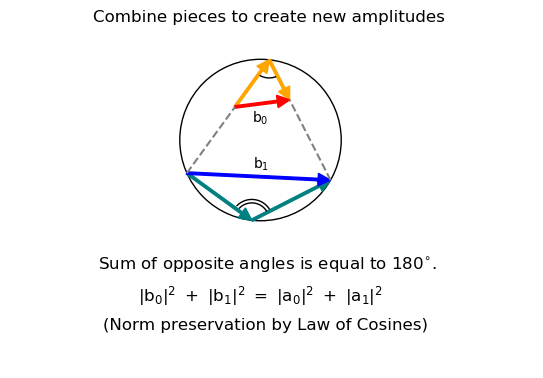
\includegraphics[trim=0 100 0 30, clip, width=\xyz\columnwidth]{./figures/fig4.png}}
	\label{fig:sigcoll}
\end{figure} 

\newpage
%\tableofcontents
%\listoffigures
%\listoftables

\section{Introduction}
This paper gives a geometric view of single-qubit quantum gates in the general case, and then explores this representation through specific single-qubit gates. The state of a single qubit is made up of two amplitudes, which are made up of complex numbers (or vectors). When a single-qubit quantum gate is applied to a qubit, the qubit’s amplitudes are scaled and added together. [Relationship with linear algebra: gates act as matrix, multiply vectors and you get scaling and addition; gates change amplitudes in the same way a matrix breaks down a 2d vector and rescales it and adds it, which lends itself well to a geometric interpretation.]  [Relationship with bloch sphere.] This paper gives a generalized geometric representation for these changes that can be applied to any single-qubit quantum gate.

\myboldhead{Why geometry?}
Amplitudes change according to the rules for scaling and adding 2d-vectors, or complex numbers.


\section{Single-qubit quantum system state}
\label{sec:state}

A quantum system is made up of a number of quantum bits, or “qubits”. Similar to a classical bit, which outputs either 0 or 1, each qubit has two outcomes when measured. This means that for a quantum system with n qubits there will be $2^n$ outcomes. Further, each of these outcomes has a corresponding probability amplitude (or vector) whose norm, when squared, gives us the probability of an outcome. From this, it follows that the sum of the squares of the amplitudes in a quantum system must equal 1, as the sum of the probabilities of all outcomes in a system must equal 1. Given the amplitudes of every outcome in a quantum state, we get a probability distribution of each of the outcomes, as in the 4-qubit state below.

\begin{figure}[hbt]
	\begin{centering}
		\ifthenelse{\equal{\onecol}{true}}{ \def\xyz{.3}}{ \def\xyz{.36}}
		\def\zyx{.005}
		{\setlength\fboxsep{0pt}\fbox{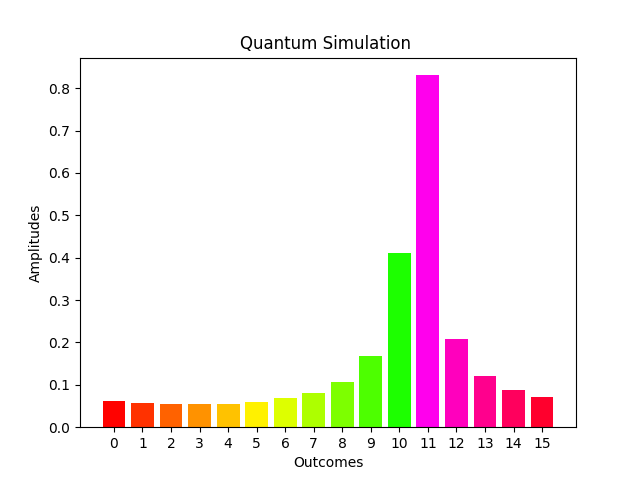
\includegraphics[width=\xyz\columnwidth]{./figures/amplitudes.png}}}\hspace{\zyx\columnwidth}
		
		\caption{Amplitudes in Quantum State.} 
		\label{fig:state}
	\end{centering}
\end{figure}
\begin{figure}[hbt]
	\begin{centering}
		\ifthenelse{\equal{\onecol}{true}}{ \def\xyz{.3}}{ \def\xyz{.36}}
		\def\zyx{.005}
		{\setlength\fboxsep{0pt}\fbox{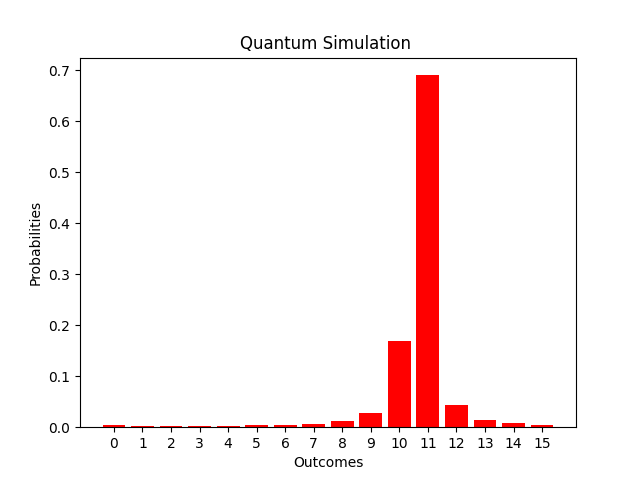
\includegraphics[width=\xyz\columnwidth]{./figures/probabilities.png}}}\hspace{\zyx\columnwidth}
		
		\caption{Probabilities in Quantum State.} 
		\label{fig:state}
	\end{centering}
\end{figure}

In this paper, the quantum state uses a single qubit. So, there are only two amplitudes (or, two vectors) in the state,
\begin{equation}
	\begin{pmatrix} a_0  \\ a_1 \end{pmatrix},
\end{equation}

with the condition $|a_0|^2 + |a_1|^2 = 1$.

  \begin{figure}[hbt]
	\begin{centering}
		\ifthenelse{\equal{\onecol}{true}}{ \def\xyz{.3}}{ \def\xyz{.36}}
		\def\zyx{.005}
		{\setlength\fboxsep{0pt}\fbox{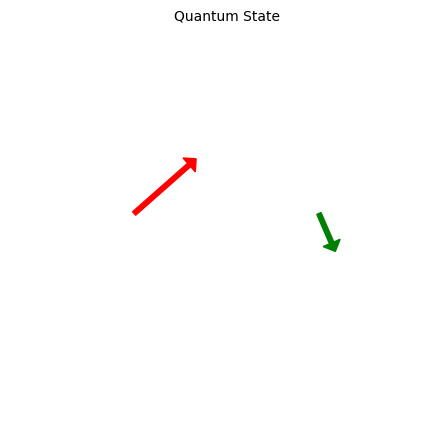
\includegraphics[width=\xyz\columnwidth]{QuantumState.png}}}\hspace{\zyx\columnwidth}
		
		\caption{Quantum State.} 
		\label{fig:state}
	\end{centering}
\end{figure}
\myvspace{-.1in}


\newpage

\section{Single-qubit quantum gates}
\label{sec:gates}
A single-qubit quantum gate is a linear transformation of two amplitudes that preserves their sum of the squared lengths. We will use the term arrows, following Feynman.

The  two arrows correspond to outcomes of a quantum computation that are identical except in the position corresponding to the target qubit. One has 0, and the other has 1 in that position. We may use the term \quot{bad} for the former and \quot{good} for the latter, and use red and green colors for their representation, respectively.

Relevant things to mention:
\begin{compactitem}
\item  general matrix form 
\item  role of $cos$ and $sin$
\item constraints, law of cosines
\end{compactitem}

\begin{equation}
	\begin{pmatrix} e^{i\alpha_0}\cos\frac{\theta}{2}  \\  e^{i\alpha_1}\sin\frac{\theta}{2} \end{pmatrix}
\end{equation}

\begin{equation}
	\begin{pmatrix} e^{i\alpha_1}\cos\frac{\theta}{2} & e^{i\alpha_3}\sin\frac{\theta}{2}\\  e^{i\alpha_2}\sin\frac{\theta}{2} &  e^{i\alpha_4}\cos\frac{\theta}{2} \end{pmatrix}
\end{equation}

$$\alpha_1 - \alpha_2  - \alpha_3  + \alpha_4 = \text{odd multiple of }\pi$$

We can restrict our attention to the case when  $alpha_1$ and $alpha_4$ are $0$, by rotating the initial amplitudes first. Describe the geometry for this case, Law of Cosines, etc.

Columns specify how current amplitudes are broken. Rows specify how new amplitudes are built.

Amplitude transformation:

\begin{equation}
	\begin{pmatrix}b_0 \\ b_1 \end{pmatrix} =
		\begin{pmatrix} e^{i\alpha_1}\cos\frac{\theta}{2} & e^{i\alpha_3}\sin\frac{\theta}{2}\\  e^{i\alpha_2}\sin\frac{\theta}{2} &  e^{i\alpha_4}\cos\frac{\theta}{2} \end{pmatrix}
	\begin{pmatrix} a_0 \\ a_1 \end{pmatrix}
\end{equation}

or, equivalently:

\begin{eqnarray*}
	b_0 = a_0e^{i\alpha_1}\cos\frac{\theta}{2}  +  a_1e^{i\alpha_3}\sin\frac{\theta}{2} \\
	b_1 = a_0e^{i\alpha_2}sin\frac{\theta}{2} + a_1e^{i\alpha_4}\cos\frac{\theta}{2}
\end{eqnarray*}


Geometrically, add scaled and rotated versions of the original amplitudes. The scaling factors are  $\cos\frac{\theta}{2}$ and $sin\frac{\theta}{2}$ for each amplitude, resulting in four pieces.

\begin{figure}[hbt]
	\begin{centering}
		\ifthenelse{\equal{\onecol}{true}}{ \def\xyz{.3}}{ \def\xyz{.36}}
		\def\zyx{.005}
		{\setlength\fboxsep{0pt}\fbox{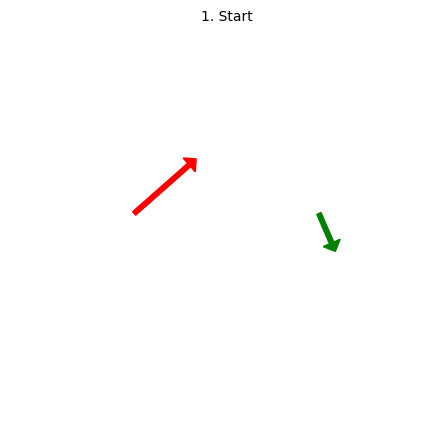
\includegraphics[width=\xyz\columnwidth]{GenericGate_step1.png}}}\hspace{\zyx\columnwidth}
		{\setlength\fboxsep{0pt}\fbox{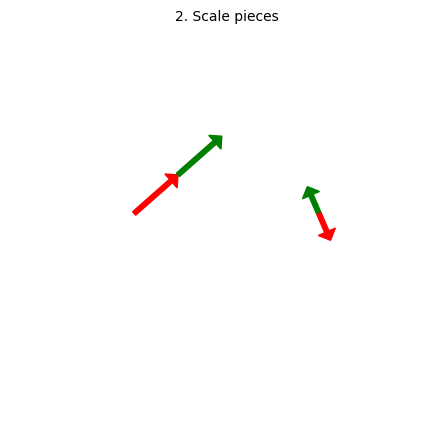
\includegraphics[width=\xyz\columnwidth]{GenericGate_step2.png}}}\hspace{\zyx\columnwidth} \\ \vspace{\zyx\columnwidth}
		{\setlength\fboxsep{0pt}\fbox{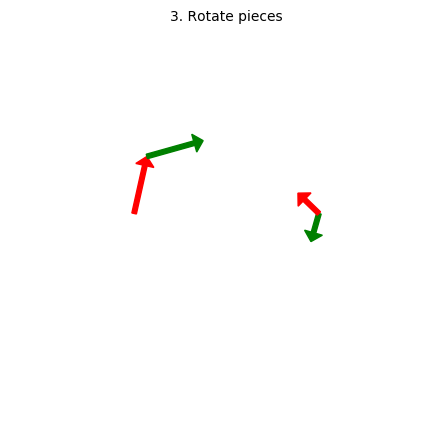
\includegraphics[width=\xyz\columnwidth]{GenericGate_step3.png}}}\hspace{\zyx\columnwidth}
		{\setlength\fboxsep{0pt}\fbox{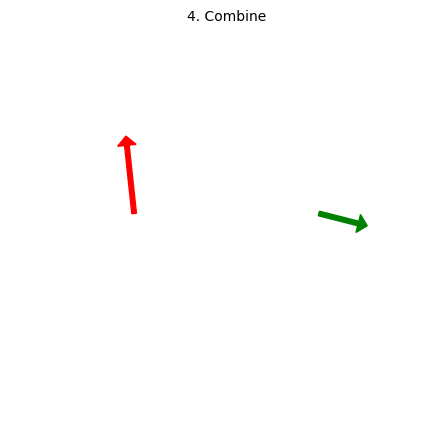
\includegraphics[width=\xyz\columnwidth]{GenericGate_step4.png}}}
		\caption{Generic Gate.} 
		\label{fig:generic_gate}
	\end{centering}
\end{figure}
\myvspace{-.1in}

\begin{figure}[H]
	\centering
	\def\xyz{1.0}
	\setlength\fboxsep{0pt}\fbox{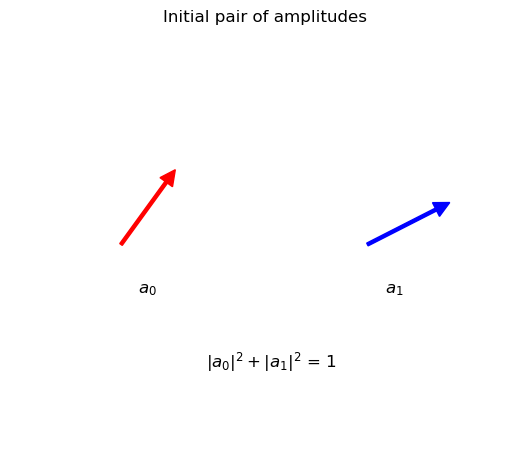
\includegraphics[trim=0 0 0 0, clip, width=\xyz\columnwidth]{./figures/fig1.png}}
	\label{fig:sigcoll}
\end{figure} 
\myvspace{-.1in}

\begin{figure}[H]
	\centering
	\def\xyz{1.0}
	\setlength\fboxsep{0pt}\fbox{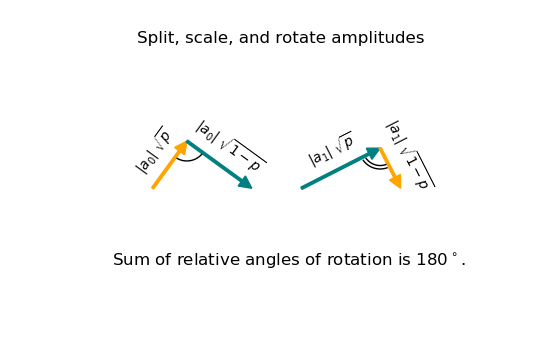
\includegraphics[trim=0 0 0 0, clip, width=\xyz\columnwidth]{./figures/fig2.png}}
	\label{fig:sigcoll}
\end{figure} 
\myvspace{-.1in}

\begin{figure}[H]
	\centering
	\def\xyz{1.0}
	\setlength\fboxsep{0pt}\fbox{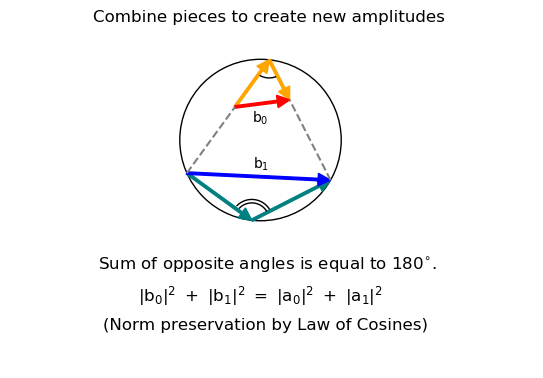
\includegraphics[trim=0 0 0 0, clip, width=\xyz\columnwidth]{./figures/fig4.png}}
	\label{fig:sigcoll}
\end{figure} 
\myvspace{-.1in}


\newpage

\section{Examples}
\label{sec:examples}
Discuss the arrow representation of some of the well-known single-qubit gates, in particular rotations.

\newpage

\subsection{Y-rotations}
$R_Y(\theta)$ for $\theta$ real.

Matrix:

\begin{equation}
	\begin{pmatrix} \cos\frac{\theta}{2} & -\sin\frac{\theta}{2}\\  \sin\frac{\theta}{2} &  \cos\frac{\theta}{2} \end{pmatrix}
\end{equation}

Amplitude transformation:

\begin{equation}
	\begin{pmatrix}b_0 \\ b_1 \end{pmatrix} =
	\begin{pmatrix} \cos\frac{\theta}{2} & -\sin\frac{\theta}{2}\\  \sin\frac{\theta}{2} &  \cos\frac{\theta}{2} \end{pmatrix}
	\begin{pmatrix} a_0 \\ a_1 \end{pmatrix}
\end{equation}

or, equivalently:

\begin{eqnarray*}
	 b_0 = a_0\cos\frac{\theta}{2} - a_1\sin\frac{\theta}{2} \\
	 b_1 = a_0sin\frac{\theta}{2} + a_1\cos\frac{\theta}{2}
\end{eqnarray*}

Geometrically, add scaled and rotated versions of the original amplitudes.
  \begin{figure}[hbt]
	\begin{centering}
		\ifthenelse{\equal{\onecol}{true}}{ \def\xyz{.3}}{ \def\xyz{.36}}
		\def\zyx{.005}
		{\setlength\fboxsep{0pt}\fbox{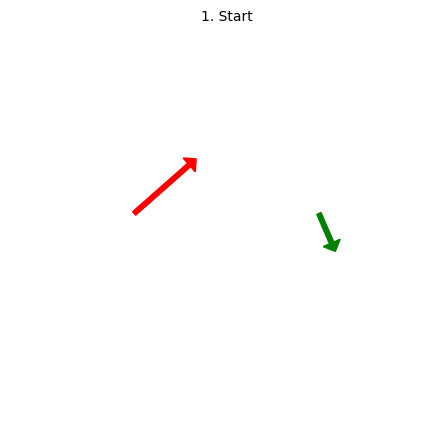
\includegraphics[width=\xyz\columnwidth]{RY1_step1.png}}}\hspace{\zyx\columnwidth}
		{\setlength\fboxsep{0pt}\fbox{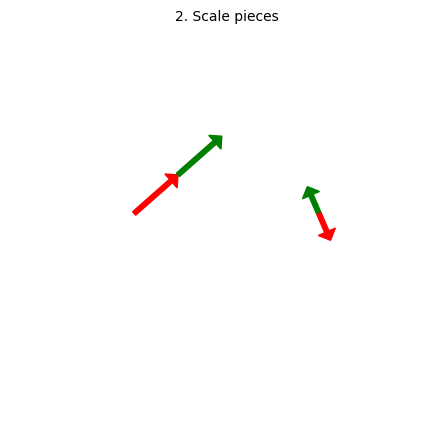
\includegraphics[width=\xyz\columnwidth]{RY1_step2.png}}}\hspace{\zyx\columnwidth} \\ \vspace{\zyx\columnwidth}
		{\setlength\fboxsep{0pt}\fbox{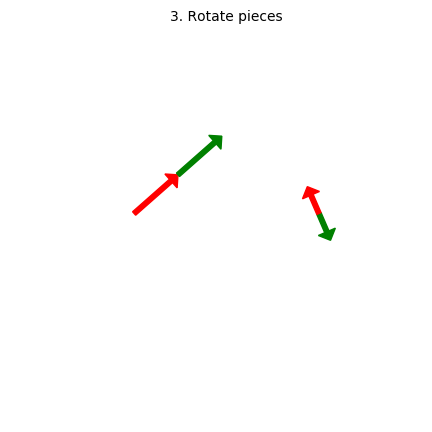
\includegraphics[width=\xyz\columnwidth]{RY1_step3.png}}}\hspace{\zyx\columnwidth}
		{\setlength\fboxsep{0pt}\fbox{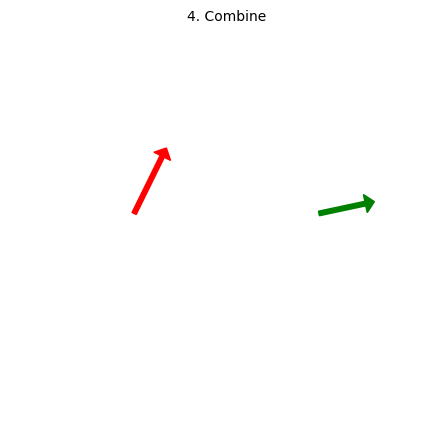
\includegraphics[width=\xyz\columnwidth]{RY1_step4.png}}}
		\caption{RY applied to a general state.} 
		\label{fig:ry1}
	\end{centering}
\end{figure}

  \begin{figure}[hbt]
	\begin{centering}
		\ifthenelse{\equal{\onecol}{true}}{ \def\xyz{.3}}{ \def\xyz{.36}}
		\def\zyx{.005}
		{\setlength\fboxsep{0pt}\fbox{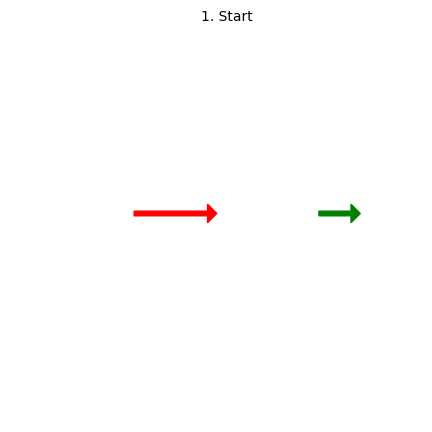
\includegraphics[width=\xyz\columnwidth]{RY_step1.png}}}\hspace{\zyx\columnwidth}
		{\setlength\fboxsep{0pt}\fbox{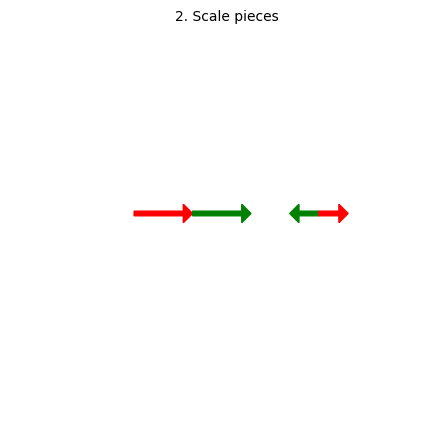
\includegraphics[width=\xyz\columnwidth]{RY_step2.png}}}\hspace{\zyx\columnwidth} \\ \vspace{\zyx\columnwidth}
		{\setlength\fboxsep{0pt}\fbox{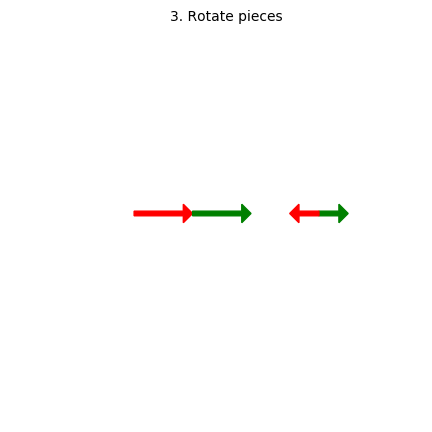
\includegraphics[width=\xyz\columnwidth]{RY_step3.png}}}\hspace{\zyx\columnwidth}
		{\setlength\fboxsep{0pt}\fbox{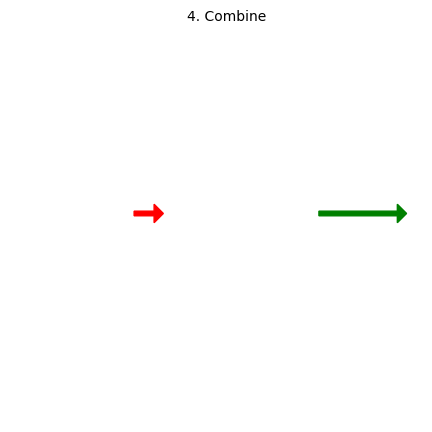
\includegraphics[width=\xyz\columnwidth]{RY_step4.png}}}
		\caption{RY applied to a state created by RY.} 
		\label{fig:ry}
	\end{centering}
\end{figure}
\myvspace{-.1in}

\newpage

\subsection{X-rotations}
$R_X(\theta)$ for $\theta$ real.

\begin{equation}
	\begin{pmatrix} \cos\frac{\theta}{2} & -i\sin\frac{\theta}{2}\\  -i\sin\frac{\theta}{2} &  \cos\frac{\theta}{2} \end{pmatrix}
\end{equation}

Amplitude transformation:

\begin{equation}
	\begin{pmatrix}b_0 \\ b_1 \end{pmatrix} =
	\begin{pmatrix} \cos\frac{\theta}{2} & -i\sin\frac{\theta}{2}\\  -i\sin\frac{\theta}{2} &  \cos\frac{\theta}{2} \end{pmatrix}
	\begin{pmatrix} a_0 \\ a_1 \end{pmatrix}
\end{equation}

or, equivalently:

\begin{eqnarray*}
	b_0 = a_0\cos\frac{\theta}{2} - a_1i\sin\frac{\theta}{2} \\
	b_1 = -a_0isin\frac{\theta}{2} + a_1\cos\frac{\theta}{2}
\end{eqnarray*}


Geometrically, add scaled and rotated versions of the original amplitudes.

  \begin{figure}[hbt]
	\begin{centering}
		\ifthenelse{\equal{\onecol}{true}}{ \def\xyz{.3}}{ \def\xyz{.36}}
		\def\zyx{.005}
		{\setlength\fboxsep{0pt}\fbox{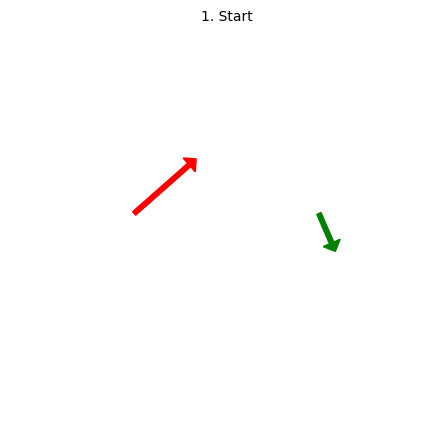
\includegraphics[width=\xyz\columnwidth]{RX1_step1.png}}}\hspace{\zyx\columnwidth}
		{\setlength\fboxsep{0pt}\fbox{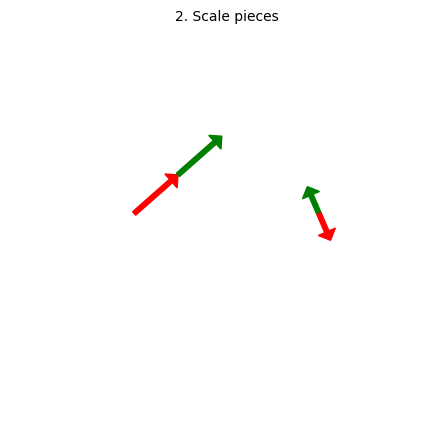
\includegraphics[width=\xyz\columnwidth]{RX1_step2.png}}}\hspace{\zyx\columnwidth} \\ \vspace{\zyx\columnwidth}
		{\setlength\fboxsep{0pt}\fbox{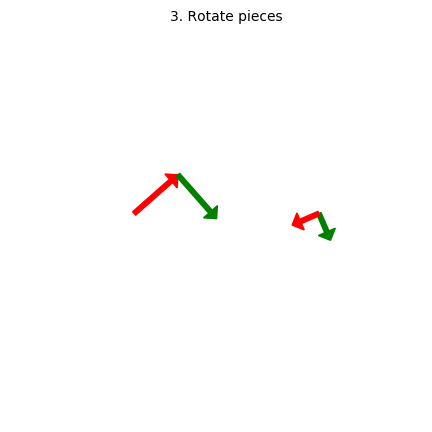
\includegraphics[width=\xyz\columnwidth]{RX1_step3.png}}}\hspace{\zyx\columnwidth}
		{\setlength\fboxsep{0pt}\fbox{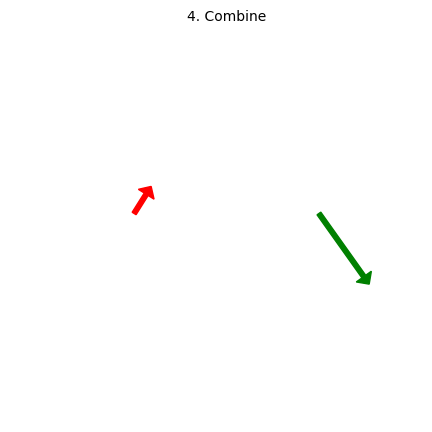
\includegraphics[width=\xyz\columnwidth]{RX1_step4.png}}}
		\caption{RX applied to a general state.} 
		\label{fig:rx1}
	\end{centering}
\end{figure}

  \begin{figure}[hbt]
	\begin{centering}
		\ifthenelse{\equal{\onecol}{true}}{ \def\xyz{.3}}{ \def\xyz{.36}}
		\def\zyx{.005}
		{\setlength\fboxsep{0pt}\fbox{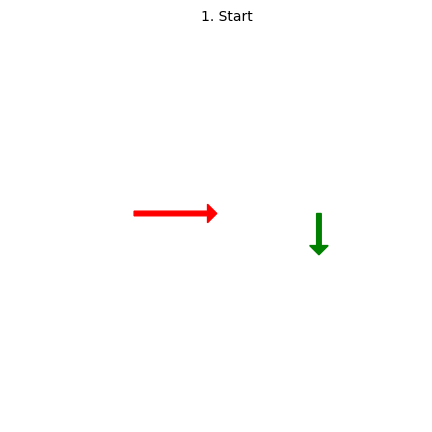
\includegraphics[width=\xyz\columnwidth]{RX_step1.png}}}\hspace{\zyx\columnwidth}
		{\setlength\fboxsep{0pt}\fbox{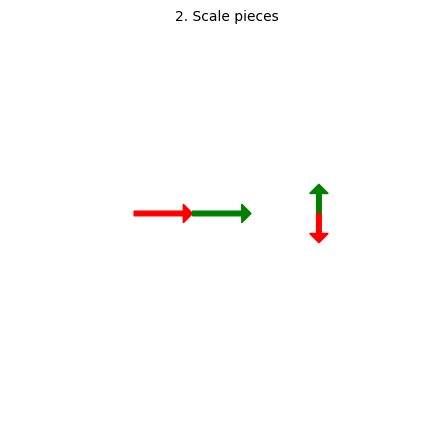
\includegraphics[width=\xyz\columnwidth]{RX_step2.png}}}\hspace{\zyx\columnwidth} \\ \vspace{\zyx\columnwidth}
		{\setlength\fboxsep{0pt}\fbox{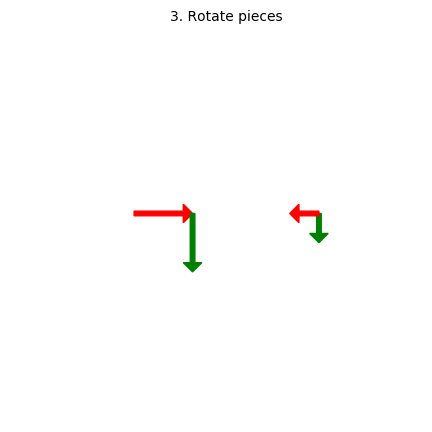
\includegraphics[width=\xyz\columnwidth]{RX_step3.png}}}\hspace{\zyx\columnwidth}
		{\setlength\fboxsep{0pt}\fbox{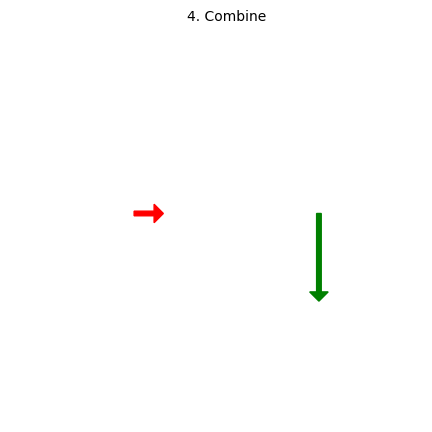
\includegraphics[width=\xyz\columnwidth]{RX_step4.png}}}
		\caption{RX applied to a state created by RX.} 
		\label{fig:rx}
	\end{centering}
\end{figure}
\myvspace{-.1in}
 
 \newpage


 \section{Inverses}
 Show how rotations of negative angles restore the original arrows.
 
  \section{Connection with the Bloch sphere}
Show connection.
 
 \section{Conclusion}
 We have established...
  \cite{gunn2017b}

%\section*{Acknowledgements} Thanks to ... for stimulating conversations and helpful feedback during the preparation of these notes.


%\section{Conclusion}

\ifthenelse{\equal{\isLong}{false}}
{}

\bibliography{ref}
\bibliographystyle{alpha}

\newpage

%\end{compactenum}
\end{document}
